%%%% For double-blind review submission, w/o CCS and ACM Reference (max submission space)
\documentclass[10pt, sigplan]{acmart}
%%\settopmatter{printfolios=true,printccs=false,printacmref=false}
%% For double-blind review submission, w/ CCS and ACM Reference
%\documentclass[sigplan,10pt,review,anonymous]{acmart}\settopmatter{printfolios=true}
%% For single-blind review submission, w/o CCS and ACM Reference (max submission space)
%\documentclass[sigplan,10pt,review]{acmart}\settopmatter{printfolios=true,printccs=false,printacmref=false}
%% For single-blind review submission, w/ CCS and ACM Reference
%\documentclass[sigplan,10pt,review]{acmart}\settopmatter{printfolios=true}
%% For final camera-ready submission, w/ required CCS and ACM Reference
%\documentclass[sigplan,10pt]{acmart}\settopmatter{}


%% Conference information
%% Supplied to authors by publisher for camera-ready submission;
%% use defaults for review submission.
%\acmConference[PL'17]{ACM SIGPLAN Conference on Programming Languages}{January 01--03, 2017}{New York, NY, USA}
%\acmYear{2017}
%\acmISBN{} % \acmISBN{978-x-xxxx-xxxx-x/YY/MM}
%\acmDOI{} % \acmDOI{10.1145/nnnnnnn.nnnnnnn}
%\startPage{1}

%% Copyright information
%% Supplied to authors (based on authors' rights management selection;
%% see authors.acm.org) by publisher for camera-ready submission;
%% use 'none' for review submission.
\setcopyright{none}
%\setcopyright{acmcopyright}
%\setcopyright{acmlicensed}
%\setcopyright{rightsretained}
%\copyrightyear{2017}           %% If different from \acmYear

%% Bibliography style

%\bibliographystyle{ACM-Reference-Format}

\citestyle{acmnumeric}   


%%%%%%%%%%%%%%%%%%%%%%%%%%%%%%%%%%%%%%%%%%%%%%%%%%%%%%%%%%%%%%%%%%%%%%
%% Note: Authors migrating a paper from traditional SIGPLAN
%% proceedings format to PACMPL format must update the
%% '\documentclass' and topmatter commands above; see
%% 'acmart-pacmpl-template.tex'.
%%%%%%%%%%%%%%%%%%%%%%%%%%%%%%%%%%%%%%%%%%%%%%%%%%%%%%%%%%%%%%%%%%%%%%


%% Some recommended packages.
\usepackage{booktabs}   %% For formal tables:
                        %% http://ctan.org/pkg/booktabs
\usepackage{subcaption} %% For complex figures with subfigures/subcaptions
                        %% http://ctan.org/pkg/subcaption
\usepackage{xspace}
\usepackage{graphicx}
\usepackage{ifthen}
\usepackage{pgfplots}
\usepackage{listings}
\usepackage{multirow}
\usepgfplotslibrary{statistics}
\usepackage{dblfloatfix} %enable fig at bottom of page
%



% Source Code
%\usepackage{color}
%\usepackage{textcomp}
%\usepackage{listings}
%\usepackage{ulem}
%\usepackage[T1]{fontenc}
%\usepackage{times}
% \usepackage{needspace}
 

% Source Code
\usepackage{color}
\usepackage{textcomp}
\usepackage{listings}

\definecolor{source}{gray}{0.85}% my comment style
\newcommand{\myCommentStyle}[1]{{\footnotesize\sffamily\color{gray!100!white} #1}}
%\newcommand{\myCommentStyle}[1]{{\footnotesize\sffamily\color{black!100!white} #1}}

% my string style
\newcommand{\myStringStyle}[1]{{\footnotesize\sffamily\color{violet!100!black} #1}}
%\newcommand{\myStringStyle}[1]{{\footnotesize\sffamily\color{black!100!black} #1}}

% my symbol style
\newcommand{\mySymbolStyle}[1]{{\footnotesize\sffamily\color{violet!100!black} #1}}
%\newcommand{\mySymbolStyle}[1]{{\footnotesize\sffamily\color{black!100!black} #1}}

% my keyword style
\newcommand{\myKeywordStyle}[1]{{\footnotesize\sffamily\color{green!70!black} #1}}
%\newcommand{\myKeywordStyle}[1]{{\footnotesize\sffamily\color{black!70!black} #1}}

% my global style
\newcommand{\myGlobalStyle}[1]{{\footnotesize\sffamily\color{blue!100!black} #1}}
%\newcommand{\myGlobalStyle}[1]{{\footnotesize\sffamily\color{black!100!black} #1}}

% my number style
\newcommand{\myNumberStyle}[1]{{\footnotesize\sffamily\color{brown!100!black} #1}}
%\newcommand{\myNumberStyle}[1]{{\footnotesize\sffamily\color{black!100!black} #1}}

\lstset{
language={},
% characters
tabsize=3,
escapechar={!},
keepspaces=true,
breaklines=true,
alsoletter={\#},
literate={\$}{{{\$}}}1,
breakautoindent=true,
columns=fullflexible,
showstringspaces=false,
% background
frame=single,
aboveskip=1em, % automatic space before
framerule=0pt,
basicstyle=\footnotesize\sffamily\color{black},
keywordstyle=\myKeywordStyle,% keyword style
commentstyle=\myCommentStyle,% comment style
frame=single,%
backgroundcolor=\color{source},
% numbering
stepnumber=1,
numbersep=10pt,
numberstyle=\tiny,
numberfirstline=true,
% caption
captionpos=b,
% formatting (html)
moredelim=[is][\bfseries]{<b>}{</b>},
moredelim=[is][\textit]{<i>}{</i>},
moredelim=[is][\underbar]{<u>}{</u>},
moredelim=[is][\color{red}\uwave]{<wave>}{</wave>},
moredelim=[is][\color{red}\sout]{<del>}{</del>},
moredelim=[is][\color{blue}\underbar]{<ins>}{</ins>},
% smalltalk stuff
morecomment=[s][\myCommentStyle]{"}{"},
%    morecomment=[s][\myvs]{|}{|},
morestring=[b][\myStringStyle]',
moredelim=[is][]{<sel>}{</sel>},
moredelim=[is][]{<rcv>}{</rcv>},
moredelim=[is][\itshape]{<symb>}{</symb>},
moredelim=[is][\scshape]{<class>}{</class>},
morekeywords={true,false,nil,self,super,thisContext},
identifierstyle=\idstyle,
}

\makeatletter
\newcommand*\idstyle[1]{%
\expandafter\id@style\the\lst@token{#1}\relax%
}
\def\id@style#1#2\relax{%
\ifnum\pdfstrcmp{#1}{\#}=0%
% this is a symbol
\mySymbolStyle{\the\lst@token}%
\else%
\edef\tempa{\uccode`#1}%
\edef\tempb{`#1}%
\ifnum\tempa=\tempb%
% this is a global
\myGlobalStyle{\the\lst@token}%
\else%
\the\lst@token%
\fi%
\fi%
}
\makeatother


%\newcommand{\ct}{\lstinline[backgroundcolor=\color{white}]}
%\newcommand{\needlines}[1]{\Needspace{#1\baselineskip}}
\newcommand{\lct}{\texttt}

\lstnewenvironment{code}{%
    \lstset{%
    % frame=lines,
    frame=single,
    framerule=0pt,
    mathescape=false
    }%
    \noindent%
    \minipage{\linewidth}%
}{%
    \endminipage%
}%


\lstnewenvironment{codeWithLineNumbers}{%
    \lstset{%
    % frame=lines,
    frame=single,
    framerule=0pt,
    mathescape=false,
    numbers=left
    }%
    \noindent%
    \minipage{\linewidth}%
}{%
    \endminipage%
}%



\newenvironment{codeNonSmalltalk}
{\begin{alltt}\sffamily}
{\end{alltt}\normalsize}



\usepackage{xcolor}
\newcommand{\todo}[1]{\color{orange}\fbox{\bfseries\sffamily\scriptsize TODO:}{\sf\small$\blacktriangleright$\textit{#1}$\blacktriangleleft$}\color{black}}
\newcommand{\egb}[1]{\color{blue}\fbox{\bfseries\sffamily\scriptsize Elisa:}{\sf\small$\blacktriangleright$\textit{#1}$\blacktriangleleft$}\color{black}}
\newcommand{\eem}[1]{\color{green}\fbox{\bfseries\sffamily\scriptsize Eliot:}{\sf\small$\blacktriangleright$\textit{#1}$\blacktriangleleft$}\color{black}}
\newcommand{\cba}[1]{\color{purple}\fbox{\bfseries\sffamily\scriptsize Clement:}{\sf\small$\blacktriangleright$\textit{#1}$\blacktriangleleft$}\color{black}}
%\newcommand*{rotatebox{75}}




% Source Code
%\usepackage{color}
%\usepackage{textcomp}
%\usepackage{listings}
%\usepackage{ulem}
%\usepackage[T1]{fontenc}
%\usepackage{times}
% \usepackage{needspace}
 

% Source Code
\usepackage{color}
\usepackage{textcomp}
\usepackage{listings}

\definecolor{source}{gray}{0.85}% my comment style
\newcommand{\myCommentStyle}[1]{{\footnotesize\sffamily\color{gray!100!white} #1}}
%\newcommand{\myCommentStyle}[1]{{\footnotesize\sffamily\color{black!100!white} #1}}

% my string style
\newcommand{\myStringStyle}[1]{{\footnotesize\sffamily\color{violet!100!black} #1}}
%\newcommand{\myStringStyle}[1]{{\footnotesize\sffamily\color{black!100!black} #1}}

% my symbol style
\newcommand{\mySymbolStyle}[1]{{\footnotesize\sffamily\color{violet!100!black} #1}}
%\newcommand{\mySymbolStyle}[1]{{\footnotesize\sffamily\color{black!100!black} #1}}

% my keyword style
\newcommand{\myKeywordStyle}[1]{{\footnotesize\sffamily\color{green!70!black} #1}}
%\newcommand{\myKeywordStyle}[1]{{\footnotesize\sffamily\color{black!70!black} #1}}

% my global style
\newcommand{\myGlobalStyle}[1]{{\footnotesize\sffamily\color{blue!100!black} #1}}
%\newcommand{\myGlobalStyle}[1]{{\footnotesize\sffamily\color{black!100!black} #1}}

% my number style
\newcommand{\myNumberStyle}[1]{{\footnotesize\sffamily\color{brown!100!black} #1}}
%\newcommand{\myNumberStyle}[1]{{\footnotesize\sffamily\color{black!100!black} #1}}

\lstset{
language={},
% characters
tabsize=3,
escapechar={!},
keepspaces=true,
breaklines=true,
alsoletter={\#},
literate={\$}{{{\$}}}1,
breakautoindent=true,
columns=fullflexible,
showstringspaces=false,
% background
frame=single,
aboveskip=1em, % automatic space before
framerule=0pt,
basicstyle=\footnotesize\sffamily\color{black},
keywordstyle=\myKeywordStyle,% keyword style
commentstyle=\myCommentStyle,% comment style
frame=single,%
backgroundcolor=\color{source},
% numbering
stepnumber=1,
numbersep=10pt,
numberstyle=\tiny,
numberfirstline=true,
% caption
captionpos=b,
% formatting (html)
moredelim=[is][\bfseries]{<b>}{</b>},
moredelim=[is][\textit]{<i>}{</i>},
moredelim=[is][\underbar]{<u>}{</u>},
moredelim=[is][\color{red}\uwave]{<wave>}{</wave>},
moredelim=[is][\color{red}\sout]{<del>}{</del>},
moredelim=[is][\color{blue}\underbar]{<ins>}{</ins>},
% smalltalk stuff
morecomment=[s][\myCommentStyle]{"}{"},
%    morecomment=[s][\myvs]{|}{|},
morestring=[b][\myStringStyle]',
moredelim=[is][]{<sel>}{</sel>},
moredelim=[is][]{<rcv>}{</rcv>},
moredelim=[is][\itshape]{<symb>}{</symb>},
moredelim=[is][\scshape]{<class>}{</class>},
morekeywords={true,false,nil,self,super,thisContext},
identifierstyle=\idstyle,
}

\makeatletter
\newcommand*\idstyle[1]{%
\expandafter\id@style\the\lst@token{#1}\relax%
}
\def\id@style#1#2\relax{%
\ifnum\pdfstrcmp{#1}{\#}=0%
% this is a symbol
\mySymbolStyle{\the\lst@token}%
\else%
\edef\tempa{\uccode`#1}%
\edef\tempb{`#1}%
\ifnum\tempa=\tempb%
% this is a global
\myGlobalStyle{\the\lst@token}%
\else%
\the\lst@token%
\fi%
\fi%
}
\makeatother


%\newcommand{\ct}{\lstinline[backgroundcolor=\color{white}]}
%\newcommand{\needlines}[1]{\Needspace{#1\baselineskip}}
\newcommand{\lct}{\texttt}

\lstnewenvironment{code}{%
    \lstset{%
    % frame=lines,
    frame=single,
    framerule=0pt,
    mathescape=false
    }%
    \noindent%
    \minipage{\linewidth}%
}{%
    \endminipage%
}%


\lstnewenvironment{codeWithLineNumbers}{%
    \lstset{%
    % frame=lines,
    frame=single,
    framerule=0pt,
    mathescape=false,
    numbers=left
    }%
    \noindent%
    \minipage{\linewidth}%
}{%
    \endminipage%
}%



\newenvironment{codeNonSmalltalk}
{\begin{alltt}\sffamily}
{\end{alltt}\normalsize}



\begin{document}

%%%
% Keyword definition (so I can change it once for all)
%%%

\def\openSmalltalkVM{OpenSmalltalk-VM\xspace}
%%%
% End Legend
%%%

%% Title information
\title[Two Decades of Smalltalk VM Development]{Two Decades of Smalltalk VM Development}
\subtitle{Live VM development through Simulation Tools}

%% Author with single affiliation.
\author{Eliot Miranda}
                                        %% can be repeated if necessary
\affiliation{
  %\position{Position1}
 % \department{VM team}              %% \department is recommended
  \institution{Feenk}            %% \institution is required
 % \streetaddress{Street1 Address1}
  \city{San Francisco}
  %\state{France}
  %\postcode{Post-Code1}
  \country{California}                    %% \country is recommended
}
\email{eliot.miranda@gmail.com}          %% \email is recommended

%% Author with two affiliations and emails.
\author{Cl\'ement B\'era}
\affiliation{
  % \position{}
	\department{Software Languages Lab}              %% \department is recommended
	\institution{Vrije Universiteit Brussel}            %% \institution is required
	\city{Brussel}
  % \state{}
  % \postcode{}
	\country{Belgium}                    %% \country is recommended
}
\email{clement.bera@vub.be}          %% \email is recommended

%% Author with two affiliations and emails.
\author{Elisa Gonzalez Boix}
\affiliation{
  % \position{}
	\department{Software Languages Lab}              %% \department is recommended
	\institution{Vrije Universiteit Brussel}            %% \institution is required
	\city{Brussel}
  % \state{}
  % \postcode{}
	\country{Belgium}                    %% \country is recommended
}
\email{egonzale@vub.be}          %% \email is recommended

%% Author with single affiliation.
\author{Daniel Ingalls}
                                        %% can be repeated if necessary
\affiliation{
  %\position{Position1}
 % \department{VM team}              %% \department is recommended
  \institution{ARCOS}            %% \institution is required
 % \streetaddress{Street1 Address1}
  \city{Aptos}
  %\state{France}
  %\postcode{Post-Code1}
  \country{California}                    %% \country is recommended
}
\email{danhhingalls@gmail.com}          %% \email is recommended

%% Abstract
%% Note: \begin{abstract}...\end{abstract} environment must come
%% before \maketitle command
\begin{abstract}

\openSmalltalkVM is a virtual machine (VM) for languages in the Smalltalk family (e.g. Squeak, Pharo) which is itself written in a subset of Smalltalk that can easily be translated to C.  Development is done in Smalltalk, an activity we call ``Simulation''. The production VM is derived by translating the core VM code to C. As a result, two execution models coexist: simulation, where the Smalltalk code is executed on top of a Smalltalk VM, and production, where the same code is compiled to executable code through the C compiler.   

%\openSmalltalkVM is a VM for languages in the Smalltalk family which is itself written in a subset of Smalltalk that can easily be translated to C.  Development is done in Smalltalk, an activity we call "Simulation", and the support code for which is "The Simulator". The production VM is derived by translating the core VM code to C, combining the generated C code with a set of platform-specific support files, and compiling with the platform's C compiler. Two execution models are effectively available, simulation, where the Smalltalk code is executed on top of a Smalltalk VM, and production, where the same code is compiled to executable code through the C compiler. Simulation is used to develop and debug the VM. Production is used to release the VM. 

%TODO egb: revisit this paragraph after reading all paper to refine problem statement and solution.
In this paper, we detail the VM simulation infrastructure and we report our experience developing and debugging the garbage collector and the just-in-time compiler within it. %We mention some of the limitations and how we worked around them. 
%We discuss specifically how we use the VM simulator to develop and debug two core VM components, the garbage collector and the just-in-time compiler. 
Then, we discuss how we use the simulation infrastructure to perform analysis on the runtime, directing some design decisions we have made to tune VM performance.

\end{abstract}

%% 2012 ACM Computing Classification System (CSS) concepts
%% Generate at 'http://dl.acm.org/ccs/ccs.cfm'.
%\begin{CCSXML}
%<ccs2012>
%<concept>
%<concept_id>10011007.10011006.10011008</concept_id>
%<concept_desc>Software and its engineering~General programming languages</concept_desc>
%<concept_significance>500</concept_significance>
%</concept>
%<concept>
%<concept_id>10003456.10003457.10003521.10003525</concept_id>
%<concept_desc>Social and professional topics~History of programming languages</concept_desc>
%<concept_significance>300</concept_significance>
%</concept>
%</ccs2012>
%\end{CCSXML}

%\ccsdesc[500]{Software and its engineering~General programming languages}
%\ccsdesc[300]{Social and professional topics~History of programming languages}
%% End of generated code


%% Keywords
%% comma separated list
\keywords{Just-in-Time compiler, garbage collector, virtual machine, managed runtime, tools, live development}  %% \keywords are mandatory in final camera-ready submission


%% \maketitle
%% Note: \maketitle command must come after title commands, author
%% commands, abstract environment, Computing Classification System
%% environment and commands, and keywords command.
\maketitle

\section{Introduction}
\label{sec:intro}

To specify the virtual machine (VM), the Smalltalk-80 team at Xerox PARC wrote a Smalltalk VM entirely in Smalltalk \cite{blueBook}. In 1995, members of the same team built Squeak \cite{SqueakByExample}, an open-source Smalltalk dialect, and its VM \cite{BackToTheFuture}, written in Smalltalk using the code from \cite{blueBook} as a starting point. Part of the code base was, however, narrowed down to a subset of Smalltalk, called \emph{Slang}, to allow Smalltalk to C compilation.  Development was done in Smalltalk, an activity we call "Simulation", and the support code for which is "The Simulator". The production VM is derived by translating the core VM code to C, combining this generated C code with a set of platform-specific support files, and compiling with the platform's C compiler. 

Two execution models were effectively available, simulation, where the Smalltalk code is executed on top of a Smalltalk VM, and production, where the same code is compiled to executable code through the C compiler. Simulation is used to develop and debug the VM. Production is used to release the VM. 
Dummy Smalltalk message sends were used to embed meta information in the code, such as \emph{self var: 'foo' type: 'char *'} which have no effect during simulation but guide the translation process of the executable Smalltalk.

When the Squeak VM was released it consisted mainly in:
\begin{itemize}
\item an interpreter with a spaghetti stack, 
\item a memory manager with a compact but complex object representation: a pointer-reversing tracing garbage collector and a heap divided into two generations,
\item WarpBlt, a rotation and scaling extension for the bit-based BitBlt graphics engine,
\item external C code and makefiles to support running the VM on popular platforms.
\end{itemize} 

The first three components of the VM were written entirely in Slang. A few extra features, such as file management, were written both in Smalltalk for simulation purposes and in C for the production VM.

Over the years, the Squeak VM evolved to give birth recently to \openSmalltalkVM\footnote{https://github.com/OpenSmalltalk/opensmalltalk-vm/}, the default VM for various Smalltalk-like systems such as Pharo \cite{PharoByExample}, Squeak \cite{SqueakByExample}, Cuis, Croquet and Newspeak \cite{NewspeakOopsla}. 
As the VM evolved, the original simulator co-evolved as a tool to develop and debug the VM. The meta data used to guide the translation process was replaced by \emph{pragmas} \cite{Pragmas}.  
%One change moved the meta data that guides translation out of the executable Smalltalk into pragmas \cite{Pragmas}.  
But the most significant evolution of the simulator came with the introduction of the Just-In-Time compiler (JIT) \cite{CogJIT}. 
%The code base was liberally sprinkled with assertions. 
The spaghetti stack was mapped to a more conventional stack frame organisation in a stack zone of a few hundred k bytes organised into small pages, a scheme called context-to-stack mapping \cite{EfficientST80}, \cite{StackMappingVW}.  Machine code generated by the JIT was executed by binding multiple processor simulators (first Bochs \cite{Bochs} for x86, SkyEye for ARMv6, Smalltalk code for 32-bit MIPS).  
Finally, a new object representation and garbage collector was added to improve performance and also to support 64-bits \cite{Forwarders}.  This required refactoring the interpreter to allow the object representation to be chosen at startup\footnote{The JIT was written with this eventuality in mind.}. Bochs was used a second time for x64 support.

One of the key design decisions in \openSmalltalkVM was to keep the core components (i.e. the interpreter, the JIT and the memory manager) written in Slang and not in C/C++.  By interpreting the Slang code as Smalltalk code, emulating native code using an external processor simulator and simulating the memory using a large byte array, it is possible to simulate the whole VM execution. This allows development and debugging of the VM with the Smalltalk development tools resulting in a live programming experience for VM development.

In this paper, we present key details of the Simulation infrastructure, give examples that demonstrate its productivity advantages, and present disadvantages that the architecture presents.
The paper is structured as follows. Section \ref{sec:VMSimulation} introduces the simulation infrastructure used to develop and debug the VM.
%In the following section, we explain the VM infrastructure with both the compilation pipeline to generate the production VM and the simulation infrastructure used to develop and debug the VM. 
Section \label{sec:Exp} reports our experience developing the VM with the simulation infrastructure. Lastly, we discuss some of the simulation limitations, the related work and conclude.

\section{Virtual Machine Simulation}
\label{sec:VMSimulation}

The key idea of the Simulation is to allow developers to reuse the whole Smalltalk IDE including the browser, inspectors and debugger to develop the VM. Most new features can be developed interactively, adding code to the VM at runtime, in the simulation environment, as for normal Smalltalk programming.

%Before detailing the simulation infrastructure used to develop and debug the \openSmalltalkVM, 
We first briefly introduce the compilation pipeline to generate the production VM and Smalltalk snapshots, key elements to understand the design of the simulation infrastructure. Then, we describe how the memory layout of both the production and simulation runtimes. In the following subsection, we explain specific aspects of the simulation infrastructure such as the simulation of the machine code generated by the JIT through the processor simulator. The last subsection discusses features related to the development of the JIT, including for example breakpoints in the machine code it generates.  

\subsection{Context}

\paragraph{VM compilation.} 
The main components of \openSmalltalkVM, the interpreter, the JIT and the memory manager, are written in Slang. The platform code, \emph{i.e.,} Operating System dependent code (such as file management or I/O), is written directly in C. 

The VM executable is generated in a two step process. Firstly, the Slang-to-C compiler translates the Slang code to C code, generating a few C files. This first step takes several seconds. Secondly, the C compiler, depending on the platform, LLVM, GCC or MSVC, translates all the C files into an executable. This second step can take up to a few minutes the first time. But, depending on what the programmer changed and what the C compiler has cached, it usually only takes a few seconds to recompile the C code. 

The VM can actually be configured in two main flavours, interpreter-only or interpreter+JIT. Although the version with the JIT is most often used in production, the interpreter version is convenient for development purposes and on devices that outlaw JITs. For example, debugging the garbage collector or evaluating new language features can be done in the interpreter-only VM, avoiding JIT complexity.

%There are multiple reasons why the core components are written in Slang and not in C/C++, being the most important VM simulation. 
%\egb{ I commented the texts on the details why you want to keep writing in Slang because they introduced noise to the explanation, and the important part is the simulation.}
%%Most of them are small details. For instance, the Slang-to-C compiler generates C code slightly different from the Slang code using different annotations. It can for example duplicate the implementation of specific methods with specific constant operands to generate more efficient code in the interpreter. 
%By interpreting the Slang code as Smalltalk code, emulating native code using an external processor simulator and simulating the memory using a large byte array, it is possible to simulate the whole VM execution. This allows development and debugging of the VM with the Smalltalk development tools resulting in a live programming experience for VM development.

\paragraph{Snapshots.}
Smalltalk is an object \emph{system}, rather than a language. The entire system, including its development tools and application code is stored in a snapshot file, which is essentially a memory dump of the entire heap. 
%A Smalltalk system is started by loading a snapshot file into a VM. The snapshot includes objects such as the classes, the compiled methods in the form of bytecodes and the running processes. At start-up, the VM restores the state of all objects in memory, swizzling pointers as required, and resumes execution in the process active when the snapshot was created.  
%A new snapshot can be made during or at the end of the session.
When programming with Smalltalk, the programmer usually starts from a snapshot which contains the core libraries, the development environment and the application under development. 
More precisely, the snapshot includes objects (such as the classes), the compiled methods in the form of bytecodes and the running processes.
Developing applications consists essentially in writing and editing code, which effectively installs, modifies and removes classes and compiled methods from objects. Programming may be done live, as the application under development is running. %, for example creating or revising methods in the debugger, and continuing. 
For example, objects may have their shape changed on the fly as instance variables are added and removed%\footnote{Code is organised in packages which are saved to an external version control system, in our case Monticello \cite{Monticello}}.
. A new snapshot can be made during or at the end of the development session.

Snapshots can be used to avoid long startup times for specific bugs. The VM can be run to a point where the bug is about to be injected, the system snapshotted, and then multiple analyses of the bug undertaken by loading the snapshot and resuming execution, either in the normal VM or in the simulator, short cutting the set up time to reach the bug.  

\subsection{Memory architectures}

\begin{figure*}[ht!]
		\centering
		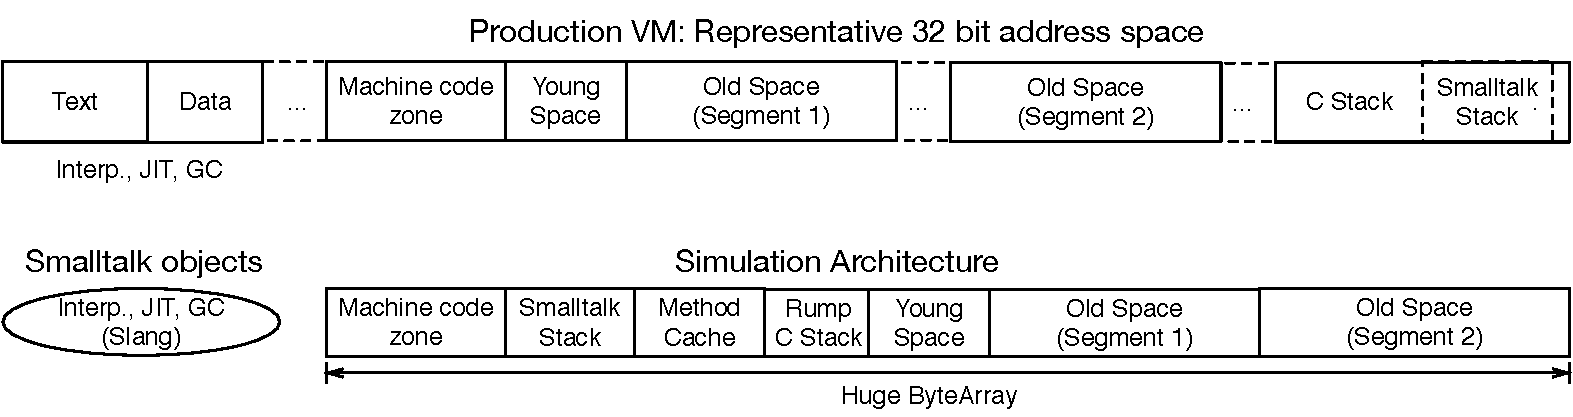
\includegraphics[width=0.9\linewidth]{figures/SimulatedMemory}
		\caption{Runtime Memory and Simulated Counter-Part}
		\label{fig:SimulatedMemory}
\end{figure*}

\paragraph{Production memory layout.}Figure \ref{fig:SimulatedMemory} describes, from a high-level perspective, the memory used by \openSmalltalkVM at runtime and the simulated counter-part. Let us detail briefly the memory used by the production VM, on the top of the figure. On the left side, which is usually the low addresses, we can first find Text, the memory section holding the native code of the VM (the interpreter, the memory manager and the JIT itself, but not the code compiled by the JIT). Then, Data holds initialized and uninitialized data, mainly the C variables used globally in the VM. 

On higher addresses, we can find the beginning of the memory managed by the VM. At start-up, the VM mmaps a memory region used for the executable code generated by the JIT (optional executable section, exists only if the JIT is enabled), for the young objects and for the old objects present in the snapshot started plus a little more space for the first \emph{tenures}\footnote{A tenure is the process of promoting young objects to old objects in a generational GC.} to be performed without triggering the full garbage collector. Later during execution, as old space grows, new memory regions are mmap'ed at higher addresses to store other old objects. 

Usually at very high addresses, we find the C stack. Room in the C stack is allocated at VM start-up to hold the Smalltalk stack zone. Both stacks are disjoint and managed differently, the stack zone being broken up into small stack pages \cite{StackMappingVW}. 

\paragraph{Simulation memory layout.}In the simulator, the heap is stored as a large contiguous byte array. References between objects are indices inside the byte array instead of pointers. All the Slang variables, normally translated to C variables, are simulated as Smalltalk objects. They use specific wrapper classes, such as \emph{CArrayAccessor} over normal Smalltalk classes, to emulate the C behavior (only array accesses are available in C, not high level iterator APIs, etc.). The Slang code is executed as Smalltalk code. The Smalltalk stack zone is represented in \openSmalltalkVM as a double linked list of stack pages which are maintained by the VM. In the interpreter-only simulator, the stack zone is a Smalltalk Array object. In the full simulator, the stack zone is in the byte array, to allow access to the stack from generated machine code by the processor simulator\footnote{This difference is historical, the interpreter-only was implemented first in the easiest way possible, but it did not work out with the JIT.}.

\subsection{Runtime simulation}

\paragraph{Modularity.}

All the Slang code is implemented in multiple Smalltalk classes, to organise the code and to add flexibility through polymorphism. For example, the \texttt{AbstractCompactor} class has two subclasses, one implementing a sweep algorithm and the other a compact one. For production, at Slang-to-C compilation time, all the code is compiled in a single C file. All the flexibility is removed, using the same example, the VM developer chooses at this moment if he wants to compile a VM with a sweep or compact algorithm. No polymorphism is available at runtime. However, since polymorphism is available in the simulator, it can be reused for debugging purposes. Still in our example, the \texttt{AbstractCompactor} class has also simulation specific subclasses. Such versions typically express additional constraints in the form of assertions which can be written in plain Smalltalk without restrictions to easily express complex constraints. They also keep specific values live so they can be accessed at debugging time.

\paragraph{JIT simulation.}

In addition to the interpreter simulator, simulating the JIT requires to simulate the execution of the native code it generates. The JIT itself is written in Slang and simulated wi th the Smalltalk execution model. To simulate the machine code, the start of the byte array representing the memory holds, when the JIT is enabled, the machine code generated at runtime. 

Bindings to processor simulator libraries (Bochs for x86 and x64, Skyeye for ARMv6, Smalltalk code for 32-bit MIPSLE) were implemented so that the machine code can be executed safely. All but the MIPSLE simulators are accessed through Smalltalk primitives.  These are effectively a combination of an FFI call to invoke foreign code plus Smalltalk code that is executed if (the code invoked by) the primitive returns an error. The next two sections describe in detail how this scheme is used to ensure that simulation and production machine code agree, how simulation machine code is interfaced to the rest of the simulation, and the debugging facilities for machine code that are available.

%Calls in-between slang code and direct machine code are a little bit trickier to simulate. Calls from machine code to slang code are implemented by using multiple invalid processor instructions, leading to a trap in the processor simulator. Such traps can be caught is the VM simulator, which then resumes Slang simulation by calling the correct method based on the invalid processor instruction. Calling machine code from Slang requires to start the machine code simulation but also to raise an exception to stop Slang simulation. Indeed, in the production VM, the processor can execute the C code or the native code generated by the JIT, but not both at the same time. 

%Machine code simulation can be performed in two different ways. The processor simulator can start simulating code until it meets an invalid instruction, or until the VM's internal heartbeat ticks. That version is convenient because it is the fastest to execute, while still catching errors such as invalid memory accesses. Alternatively, it can simulate one instruction at a time. This second version is slower, but it allows to implement specific debugging features, such as conditional breakpoints in-between each machine instruction.

\paragraph{Deterministic simulation.}

To be able to reproduce the same bug the exact same multiple times in a row, we designed the simulator to be as deterministic as possible. The most important things to note are the following:
\begin{itemize}
\item Simulated memory is not subject to Address Space Layout Randomisation,
\item A synthetic clock is used so that time advances in lock step with code execution.
\end{itemize}

\paragraph{Interfacing machine code with simulation objects.}

A key requirement to enable effective development of the JIT is that the code generated during simulation be as close as possible to the code generated by the production JIT.  The code is of course not bit-identical; the address space is laid out very differently in memory to the simulation's byte array and the simulator is not subject to Address Space Layout Randomisation. But we benefit from the code generated under simulation being otherwise identical to that generated in the production VM and we go to some effort to achieve this.  The technique we use, involving illegal addresses, also allows us to interface the Smalltalk objects that comprise the Simulation, the interpreter, memory manager and jit, and variables within them, with machine code. To explain this let's consider how the interpreter references a stack frame.

The interpreter has framePointer, stackPointer and instructionPointer variables used to interpret code. When machine code wants to enter the run time, for example to have the run time look up a send, or to invoke the scavenger when eden is full, it needs to record the current stack frame, writing the native stack and frame pointers into the stackPointer and framePointer variables, and then to call the relevant routine in the run time. The run time can then access the current machine code stack frame though these variables.  In the production VM, the stackPointer and framePointer variables are C variables at known addresses in Data, and routines in the runtime have been compiled from C and exit in Text.  Referencing these variables and invoking runtime routines from machine code is therefore straight-forward.  But in the simulation they are inaccessible.  First of all they are instance variables inside Smalltalk objects, objects that have strong encapsulation, accessible only through messages, and second of all they are alongside the simulation's byte array, not within it, therefore the processor simulator has no access to these variables.

\todo{Shorten and abstract next paragraph. }

The JIT maintains a set of Dictionaries (hash maps) that map integers representing addresses to closures that get or set variables in the simulation objects, or invoke runtime routines, in both cases by sending messages to the simulation objects.  As code is JITted and specific variables and runtime routines are referenced the JIT manufactures a unique illegal address to reference the variable or routine, and uses this as the key in the relevant map, creating and storing the relevant closure accessor as the value.  When the processor simulator attempts to execute an instruction containing one of these illegal addresses, which will be some variety of read, write, call, jump or return instruction \footnote{activations of JITted machine code methods return to calling interpreter frames by returning to a trampoline that transfers control to the interpreter; hence the return address of a machine code activation above an interpreter frame has this trampoline as its return address}, it will attempt to raise an exception.  Our processor simulators are invoked through a "primitive" interface, much like an FFI call, and the attempt to raise an exeption is caught by wrapper code that returns an error result from the primitve invocation; in Smalltalk terminology the primitive fails.  The primitive failure code, Smalltalk code in the method that contains the primitive invocation, then analyses the offending instruction and constructs a Smalltalk ProcessorException object.  This Smalltalk exception has a type (\#read, \#write, \#jump, \#call), the address of the memory location being read, written, jumped to or called, a program counter (pc) holding the instruction's address, a next pc, and an accessor for the register, if any, that is the target of the read or the source of the write.  The processor simulator is invoked in the context of an exception handler for ProcessorException exceptions which invokes a Smalltalk method, handleSimulationTrap:, that invokes the relevant closure.  Once the closure has completed, the processor simulator is advanced to the nextpc and simulation resumes.  In this way, machine code generated in simulation can access arbitrary simulation objects while remaining essentially identical to the generated machine code in the production VM. Further, ProcessorException, and a handful of other methods implemented by a processor simulator makes the interfacing of machine code to the Smalltalk part of the simulation portable and processor independent.

\subsection{Machine code debugging}

\paragraph{Instruction recording.}

The JIT maintains a simulation-only variable that determines whether the processor simulator is invoked in single-stepping mode, or run-until-exception-or-interrupt mode.  When in single stepping mode a circular buffer remembers N previous instructions and associated register state, allowing one to examine an arbitrary number of instructions (by default 160) preceding some error. The breakpoint facility is intelligent enough to only enable single stepping once code has been JITted at that address, using run mode until that point.

\paragraph{Conditional breakpoints.}

\todo{Rework. maybe check interaction with section JIT debug.}

There is a small polymorphic scheme for breakpoints.  Booleans, integers, and arrays understand isBreakpointFor: pc.  So if the breakPC object is false there is no breakpoint.  If the breakPC is true then any pc is a potential breakpoint.  If it is an integer then that pc is a potential breakpoint.  If the pc is an Array then the pc is a breakpoint if any value in the array answers true to isBreakpointFor:.  The scheme could trivially be extended to include intervals.  If breakPC isBreakpointFor: pc is true then the breakBlock is sent shouldStopIfAtPC: pc.  booleans and closures understand shouldStopIfAtPC:.  true and false make the breakpoint unconditional or disabled respectively, and a closure evaluates itself, allowing one to specify arbitrarily complex breakpoints.  For example, one can specify that execution should stop at a particular pc if the top two elements on the stack satisfy some criterion.  It is much more powerful and much simpler to use than typical machine-level debuggers, and it can be extended as one is debugging (for example, adding interval support during the middle of a debugging session if required).

\paragraph{In-image compilation.}

\todo{Merge 1 and 2 + some shortening}

%1

Each processor simulator is expected to be able to disassemble its machine code.  The Smalltalk code for each processor simulator implements a simple parser that identifies constants and field offsets embedded in machine code and passes these to routines in the JIT and the interpreter that lookup addresses, matching them to objects, in particular message selectors and classes, and to method local variable names, rendering the machine code much more readable than machine code displayed in a typical machine oriented debugger.  For example, here is a snippet of decorated disassembly for x64:

\lstdefinelanguage
   [x64]{Assembler}     % add a "x64" dialect of Assembler
   [x86masm]{Assembler} % based on the "x86masm" dialect
   % with these extra keywords:
   {morekeywords={movq, cmpq, %
                  rax,rdx,rcx,rbx,rsi,rdi,rsp,rbp, %
                  r8,r8d,r8w,r8b,r9,r9d,r9w,r9b, %
                  r10,r10d,r10w,r10b,r11,r11d,r11w,r11b, %
                  r12,r12d,r12w,r12b,r13,r13d,r13w,r13b, %
                  r14,r14d,r14w,r14b,r15,r15d,r15w,r15b}} % etc.

\lstset{language=[x64]Assembler}

\begin{lstlisting}
00002063: movq 0x800(%rbx), %rax = 'stackLimit' : 48 8B 83 00 08 00 00 
0000206a: cmpq %rax, %rsp : 48 39 C4 
0000206d: jb .-0x47 (0x2028=indexOf:startingAt:ifAbsent:@28) : 72 B9 
HasBytecodePC bc 40/41:
0000206f: movq start@20(%rbp), %rsi : 48 8B 75 14 
00002073: movq anElement@28(%rbp), %rdi : 48 8B 7D 1C 
00002077: movq self@-12(%rbp), %rdx : 48 8B 55 F4 
0000207b: movq $0x0, %rcx : 48 C7 C1 00 00 00 00 
00002082: call .-0x1B2F (0x558=ceSend2Args) : E8 D1 E4 FF FF 
IsSendCall indexOf:startingAt: bc 44/45:
00002087: movq %rdx, index@-20(%rbp) : 48 89 55 EC 
\end{lstlisting}

\todo{RM end of next paragraph or ref}

This code is the end of the entry sequence that checks the stack pointer against the stack limit for the end of the current stack page, which is also used to break out of machine code to service interrupts or events such as invoking the scavenger, etc.  \emph{\%rbx} is used as a base register pointing at the variables in interpreter.  Following that is the code for \emph{index := self indexOf: anElement startingAt: start} where \emph{anElement} and \emph{start} are method parameters and \emph{index} is a local variable.  HasBytecodePC and IsSendCall are decorations that identify important locations in machine code, including object references, runtime calls, etc. These points are specified using metadata implemented as a simple bytecoded language, a stream of such bytes being added to the end of each machine code method.  This metadata is parsed when the garbage collector needs to locate object references in machine code, when linked sends must be relocated when the machine code zone is compacted to make space by throwing away some number of least recently used methods, and when machine code pcs must be mapped to their corresponding bytecode pcs to preserve the illusion that the VM is a bytecode interpreter using a spaghetti stack of Context objects.

%2

Simulating the whole VM requires going through the whole start-up sequence: loading the snapshot, running code registered in the start-up sequence and resuming the user interface. The whole start-up takes around 15 seconds on a recent Macbook pro. While developing the JIT, this start-up time may still be too long and move the live programming experience to an edit-compile-run cycle, which we want to avoid.  Further, a particular method that exercises some new part of the JIT may be problematic to have executed suring simulation and hence not easily JITted during simulation.

To work around these problems, we implemented a tool called \emph{In-image compilation}. In-image compilation allows invoking the JIT as a Smalltalk library on any bytecode compiled method in the host Smalltalk system (i.e. \emph{not} in the simulated heap) to generate the corresponding machine code. In-image compilation invokes the JIT on the method, calls the bound processor simulator to disassemble the code and decorate the disassembly and then dumps the output in a text window. Indeed the above snippet is from an in-image compilation.  To generate the machine code, the JIT has to access specific objects (the compiled method, the literals, known objects such as true, false or nil) as if they were in the simulated memory. To implement this we built a facade, which masquerades as the simulation's memory manager, and translates the state of the bytecode compiled method in the current simulation into state that makes it appear as if it were resident in a simulaiton byte array.  This includes mock addresses for all the object the JIT may require to generate the machine code of a given method. Figure \ref{fig:InImageCompiler} summarizes the process. Note that this technique applies for the baseline JIT, which translate a single bytecode method into machine code, adaptive optimizations and speculative optimizations are debugged differently.


\begin{figure}[ht!]
		\centering
		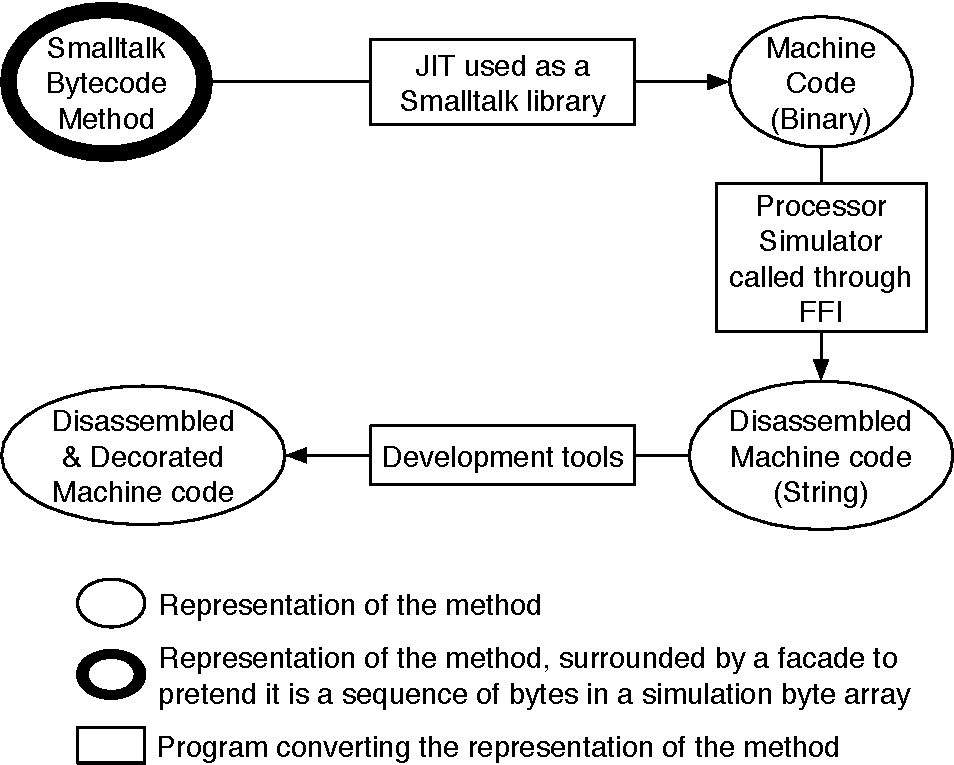
\includegraphics[width=\linewidth]{figures/InImageCompiler}
		\caption{In-image compilation}
		\label{fig:InImageCompiler}
\end{figure}

\paragraph{Templates.} The JIT generates a sequence of machine instructions for a given pattern of bytecodes. We use the term template to describe the sequence of machine instructions generated for a pattern of bytecodes, even though we do not like to reduce the JIT to a simple template-based JIT since each bytecode generates slightly different machine instructions based on register pressure, a simulated stack and  
a few heuristics. Since the JIT is template-based, in-image compilation is very convenient to develop and optimize each of the JIT templates. 

Since we also have a bytecode assembler that allows us to manufacture bytecoded methods we can in practice exercise any part of the JIT by creating a suitable bytecoded method from the assembly code.  Although for methods of the complexity produced by the adaptive optimiser this is hardly pleasurable.

\section{Experience reports}
\label{sec:Exp}

\todo{add intro about this is anecdote and examples of how we used it ; fix section }

\subsection{Implementing a new full GC algorithm}

\todo{Remove Assertion references}
\todo{Make it more like a story like the following 2 subsec}
Recently, to evaluate new old space garbage collection algorithms we designed against standard algorithms, we implemented a Mark-Sweep in addition to the existing Mark-Compact collector. The whole implementation was done in the simulator, and only when it was working there, was it compiled to C. Using this process, the compiled C code was kind of working out of the box. To describe the implementation process, we need to discuss briefly first the assertion levels in the VM. Then we will show how we debugged the algorithm.

%\paragraph{Assertions.}To stabilise our code base and find easily production bugs, all the code based is annotated with assertions. Each assertion ensures a specific state is as the VM developer would expect it to be and stops or log the incorrect result if not. We have a multi-level assertion system. Assertions written in plain Smalltalk are convenient since more complex constraints can be expressed easily using high level structures (Sets, etc.), but they can be performed only in the simulator. Assertions written in Slang are executed in the simulator but they are also compiled to C. The C compiler, based on a compilation flag, chooses to compile the VM with or without assertions. The VM with assertions is used for debugging and to recreate snapshots just before a VM crash. The VM without assertions is the production VM.


\paragraph{Simulation.} Once we had partially written the new Sweep algorithm, we started the simulator. Since the algorithm was partially written, we had to write the missing pieces inside the debugger, installing the new code at runtime, as one can do it in any Smalltalk application. In addition, the simulator has an interesting property: each time it performs a GC, either a scavenge or an old space collection, it first copies the simulated memory (\emph{i.e.,} the heap), performs the GC there, and if no assertion fails, it then performs the GC on the original version. This means that if the algorithm was not working, and likely an assertion would fail or an error such as incorrect memory access would be raised, the erratic behavior would have happened in a copy of the heap. The simulator can then reproduce the exact same erratic behavior as many times as the VM developer wants duplicating again and again the same original heap. This is very convenient to debug specific GC bugs. Indeed, often in GC bugs, when the bug happens, the memory is already corrupted and it's quite difficult to track back where the bug comes from without rewinding the memory state, which is usually very difficult or impossible.

%We firstly discuss how we use the simulator to debug crashes in deployed applications, then how we use in-image compilation to develop the JIT itself.

\subsection{Debugging a crash in machine code with conditional breakpoints}

In the recent years, we added support for a more aggressive JIT with speculative optimizations through a bytecode to bytecode optimizer \cite{SistaFastStartUp}, re-using the existing template JIT as a back-end. To be able to generate efficient bytecodes in the bytecode to bytecode optimizer, we had to introduce new unsafe bytecodes allowing, for example, accesses in arrays without any checks (type and bounds checks) \cite{SistaBytecodeSet}. For each new bytecode, we introduced new templates in the existing JIT to generate efficient machine code for the optimized methods using the new bytecodes. Once all the basic unit tests worked, we ran the VM with the speculative optimizer, which executed optimized code, and got a crash. We could figure out which bytecode method was triggering the crash, but we had no idea from which template the crash came from. In addition, optimized methods include many inlined methods, making them very large, so it was difficult to figure out where the issue comes from just by looking at thousands of bytecodes.

To understand the crash, we created a snapshot where the faulty method was executed right after start-up. We started the VM simulator, and set-up a conditional breakpoint so that simulator would stop when the JIT would generate that method to machine code. Then, when the simulator effectively stopped, we changed the conditional breakpoint to stop execution when the address corresponding to the faulty method entry in machine code would be used, either by a call from the interpreter or through inline cache relinking. The simulator stopped again, about to execute the machine code corresponding to the faulty method. We then cloned the simulator to be able to reproduce the crash again and again.

Executing the faulty method led to an assertion failure. However, that assertion failed in a GC store check, telling us that the object to store into looked suspicious (address outside of the heap). It happens that this object was read from a field on stack, and that this field held an incorrect address. We could not tell anymore at this point in the execution what instruction among the thousands previous ones wrote on stack the invalid address. So we discarded the cloned simulation, and cloned a fresh simulator again, just before the execution of the faulty method in machine code to reproduce again the crash. This time, we enabled single stepping (\emph{i.e.,} the processor simulator simulates one instruction at a time) and we added a breakpoint stopping execution when the specific field on stack would be written to the incorrect value found before. In this case, the conditional breakpoint is checked in between each machine instruction, and execution stopped right after the machine instruction which wrote the incorrect value on stack. From the machine instruction address, we could figure out which bytecode pattern generated the incorrect machine code (it was the new bytecode template for inlined allocations). From there, we built a simpler method crashing the runtime and fixed the template using in-image compilation (See next subsection). 

The debugging process discussed here is exampled in a youtube video\footnote{https://www.youtube.com/watch?v=hctMBGAXVSs}.

\subsection{Optimizing the store templates with in-image compilation}

A few years ago, we added support in the VM for read-only objects \cite{ROObject}. Read-only objects were critical performance-wise for specific customers using them in the context of object databases. To maximize the performance, we changed the templates in the JIT compiler for the different memory stores. %Since the JIT has to generate very quickly machine code, it goes through the code three times: (1) it scans the bytecode, (2) it generates abstract instructions from the bytecode and (3) it generates the native instructions from the abstract instructions. The abstract instructions are mapped almost one to one to machine instructions, their main purpose is to compact the generated code by removing Nops used for jump targets or finding out out the size of jumps.
To optimize each template, we use the in-image compilation framework. We selected a method with a single store to make it simple. We requested the JIT to generate the machine code and changed the template to optimize until the machine code generated was the exact instructions we wanted. It is possible, in in-image compilation, to use the Smalltalk debugger on the JIT code itself to inspect the JIT state and fix the JIT code on-the-fly without any major compilation pause. Once we went through the few store templates (there are a few different templates for optimizations purposes, for example, storing a constant integer does not require a garbage collector write barrier check), we've just had to evaluate performance and correctness through benchmarks and tests to validate the implementation.

\subsection{Machine code zone send analysis}

\todo{Make following 2 subsections more like a story like the previous ones}

A side-effect of VM simulation, and specifically to be able to interrupt the simulation and introspect the simulated memory and simulation specific objects, is to be able to analyse the runtime with scripts written on-the-fly. Indeed, the simulator can be stopped at any given point and arbitrary Smalltalk code can be written and evaluated similarly to the \emph{eval} Javascript construct to analyse the simulated memory, including the machine code zone, the heap or any Smalltalk object representing the VM state.

One of the first analysis we ran was on the machine code zone. We stopped the simulation when the machine code zone reached 1Mb. We then iterated over it and investigated what was in. As show in Table \ref{tab:generalAnalysis}, 1752 methods were compiled to machine code by the JIT, 6352 sends\footnote{We use the Smalltalk terminology, send, to discuss virtual calls since we are talking about Smalltalk.} are present but 2409 of them are not linked (basically, they have never been used). 

\begin{table} [th]
\centering
\begin{tabular}{l|r}
	Number of methods  & 1752 \\
  \hline
	Number of sends  &  6352 \\
  \hline
	Average number of sends per method  & 3.63  \\
  \hline
	Number of unlinked sends  &  2409 \\
  \hline
	Percentage of unlinked sends  & 37.9\%  \\
  \end{tabular}
\caption{General Machine Code Zone Analysis\vspace{-0.5cm}}
\label{tab:generalAnalysis}
\end{table}

Further analysis, in Table \ref{tab:polyAnalysis}, confirms Urs H\"{o}lzle statement \cite{PICSelf}: around 90\% of used send sites are monomorphic, around 9\% are polymorphic (up to 6 different cases in our implementation) and the remaining \% is megamorphic.

\begin{table} [th]
\centering
\begin{tabular}{l|c|c}
  	& Number of sends & \% of linked sends \\
  \hline
	Monomorphic & 3566 & 90.4 \% \\
	Polymorphic & 307 & 07.8 \% \\
	Megamorphic & 70 & 01.8 \% \\
  \end{tabular}
\caption{Polymorphism Inline Cache Analysis\vspace{-0.5cm}}
\label{tab:polyAnalysis}
\end{table}

The code used for these analysis is detailed in the Section "Let Me Tell You All About It, Let Me Quantify" of the blog post "Build me a JIT as fast as you can"\footnote{http://www.mirandabanda.org/cogblog/2011/03/01/build-me-a-jit-as-fast-as-you-can/}.

\subsection{Directing VM optimizations through analysis}

The results of the analysis are sometimes used to direct performance design decisions on the VM. In this section we describe how the analysis impacted a design called "Early polymorphic inline cache promotion".

We designed the polymorphic inline caches (PICs) \cite{PICSelf} with two implementations:
\begin{itemize}
	\item \emph{Closed PICs:} Such caches can deal with up to 6 cases, and are basically implemented as a jump table.
	\item \emph{Open PICs:} Such caches can deal with any number of cases, they consist of three probes searching the global look-up cache (a hash map shared with the interpreter) and fall back into a standard look-up routine if nothing is found after three attempts.
\end{itemize}	

One idea we had was to promote a monomorphic inline cache straight to an open PIC if available, and create the closed PIC only if no open PIC is available for the given selector. The benefit is avoiding lots of code space modifications and an allocation. The downside is replacing faster closed PIC dispatch with slower open PIC dispatch. The question is how many send sites would be prematurely promoted to megamorphic, or how many closed PICs have selectors for which there are open PICs.

The analysis result showed that 17\% of polymorphic send sites would get prematurely promoted. So we have implemented a simple sharing scheme. The JIT maintains a linked list of open PICs, and before it creates a closed PIC for a send site it will patch it to an open PIC if the list contains one for the send's selector.

Analysing the question is easy in our context.  This analysis took about an hour to perform, including writing an iterator over send sites, and then implementing the eager promotion to open PICs.  Somewhat similar analyses one of the authors performed on the second generation Deutsch Schiffman VM \cite{EfficientST80}, which is written entirely in C, when adding the same PIC scheme took several days, having to be written statically and tested with a traditional edit-compile-debug cycle. The productivity difference is extreme.

\section{Discussion and Related Work}

\subsection{Virtual Machine simulation limitations}

\todo{Merge 1 and 2}

%1
\paragraph{Interpreter-only simulation.} 
 Since executing machine code on the processor simulators is not fast, the simulated interpreter may be faster \footnote{but JIT code is so much more optimized than bytecode interpretation that it may indeed be faster, depending on the code being executed}, and startup time and memory footprint are smaller.
 
 %2
 
 The simulator has several limitations. Due to the simulation infrastructure being different from the actual hardware, code is run differently and one could think it leads to strange bugs happening only in simulation or in production. However, we have been using this infrastructure since 1995, and these kinds of bugs are really rare and usually easy to fix. We have however two main limitations: simulation performance which is quite slow and calls to external C/C++/machine code which cannot (yet) be simulated.

\paragraph{Performance.}
The first limitation is due to the simulation performance. The interpreter-only is simulator is around 200 times slower to execute code than the normal VM. With the JIT and processor simulation enabled, without specific debugging options such as conditional breakpoints in between machine instructions, simulation drops to around 500 times slower than the normal VM. We usually enabled conditional breakpoints in-between machine instructions only when we reach a point in the simulator where the bug is about to happen since it is way slower, so the overall performance in this context is not really relevant.

This means for example that if a GC bug happens in an application 15 minutes after start-up, it will take 50 hours to reproduce in the interpreter-only simulator. Bugs in the jitted code are worse. Fortunately, we work around this problem by using snapshots and the interpreter-only simulator for GC bugs. In general, once we are able to reproduce a bug in the production VM, we try to snapshot the runtime just before it crashes. The VM simulator can then be started just before the crash and the debugging tools can be used after only several dozens of seconds. If the bug is unrelated to the JIT, the interpreter-only simulator can also be used and it is a little bit quicker to execute code.

\paragraph{Calls to external code.}
Although most of the GC and JIT development and debugging can be done in the simulator, specific tasks cannot be done this way. Basically, any calls outside of the machine code generated by the JIT and the Slang code cannot be simulated. For specific small parts of the VM, such as file management, we extended the simulator, effectively duplicating the code base with the C code, to support those features in simulation. However, there is no solution in the general case: we cannot afford to simulate both the compiled C code and the jitted code on the processor simulator, that would be horribly slow, and specific behaviors in the machine code not present in the code generated by the JIT can hardly be simulated (Access to C variables, OS variables, etc.).

The main limitation we have right now is with Foreign Function Interfaces (FFI). We have a significant amount of bugs in FFI, often due to specific interaction between call-backs, low-level assembly FFI specific glue code and moving objects. Such bugs cannot be debugged with our simulation infrastructure so far and we have to rely on gdb/lldb.

\subsection{VM Simulator and Bootstrapping facilities}

In general, the simulator provides a toolkit for manipulating and inspecting snapshot files.
  Snapshots can be used to avoid long startup times for specific bugs.  A simulation can be run to a point where the bug is about to be injected, the system snapshotted, and then multiple analyses of the bug undertaken by loading the snapshot and resuming the simulation, short cutting the set up time for the simulator.  
  %Simulation is of the order of a thousand times slower than actual execution.

%shorteinig the miscellaneous uses.
Besides being a key tool in VM development, the simulator can be used to indirectly allow the VM to be started from source files ~\cite{PharoBootstrap}. The simulator is also used to create 64-bit images from 32-bit images, a transformation that involves replacing certain instances of classes by certain others (e.g. in the 32-bit system all floats are 8 byte boxed objects while 64-bit systems support an immediate floating point type that represents a subset of 64-bit IEEE 754 floating point numbers).

\subsection{Related Work}

Many VM developers implemented different tools to help them working more efficiently on their VM, but they rarely publish about it. This section focuses on the two closest related works.

\todo{We need to mention something about graal, maybe high level lang for VM and debugging in general then refs}

\paragraph{Maxine Inspectors.} The Maxine inspectors \cite{MaxineInspector} were demonstrated at OOPSLA'18. They allow to inspect the running state of the Maxine VM while it runs for debugging purposes. One of the main difference with our design is that the Maxine VM is metacircular, hence it does not have a simulation and a production mode as we do but a single production debuggable mode. We believe having two different modes allows us to easily generate a production VM while still having nice debugging features. Having a full metacircular VM would be interesting, but it is unclear whether it is convenient to build a production VM in that way. So far, most production VMs (Java, Javascript, etc.)are still compiling through the C/C++ compiler and are not metacircular

%However, so far, most production VMs (Java, Javascript, etc.), even after the huge recent investments in the Javascript VMs by the four major web vendors, are still compiling through the C/C++ compiler and are not metacircular. 
%Hence, although a metacircular VM has interesting advantages, it is not clear it is that convenient to build a VM in such a way.

\paragraph{RPython toolchain.}  The RPython toolchain \cite{RPythonToolchain} was designed and implemented quite similarly to \openSmalltalkVM. Most of the VM code is written in RPython, a restricted Python, instead of Slang, and some leftovers are written in plain C. RPython is, however, much closer to Python than Slang is to Smalltalk. 
%RPython allows higher-level structures such as dictionaries to be used. 
%The design decision comes with its set of advantages and drawbacks. 
The key advantage of such a design choice is that the RPython code feels like Python code and is relatively quite easy to read write, unlike Slang which feels like C and is as easy to write as C. The main drawback is that RPython to C compilation takes way longer than the Slang to C compilation (up to 40 minutes in a recent Macbook pro for the RSqueak VM \cite{RSqueak}, instead of several seconds for Slang). 

Although the RPython code can be executed as normal Python code, the developers seem to think it is not worth to do such a thing, mostly because executing code in this way is very slow. 
The overall architecture of the RPython toolchain is different, resulting in a longer time to reach peak performance (though their peak performance is at least in theory better than with our JIT). This time may be quite significant in simulation mode. In contrast, in \openSmalltalkVM, we can reuse the snapshots to work around the simulation slow performance.

%In addition, RPython was originally designed for Python, which does not feature snapshot by default, so they cannot abuse snapshots to work around the simulation slow performance.

\section*{Conclusion}

This paper introduced and discussed the \openSmalltalkVM simulation infrastructure, used to develop and debug the VM. In particular, we described our experiences developing and debugging the full garbage collector and the JIT compiler. We believe Simulation is a powerful tool allowing us to reduce the development time and to fix bugs quickly. 

In the near future, we plan to extend the simulator with customizable development tools. Currently the tools built in top of the simulation infrastructure are mainly textual. More advanced tooling such as the moldable inspectors and debuggers \cite{MoldableInspector, MoldableDebugger} should enable a more interactive interface, making it easier to apprehend by new developers.

%% Acknowledgments
%%\begin{acks}                            %% acks environment is optional
                                        %% contents suppressed with 'anonymous'
  %% Commands \grantsponsor{<sponsorID>}{<name>}{<url>} and
  %% \grantnum[<url>]{<sponsorID>}{<number>} should be used to
  %% acknowledge financial support and will be used by metadata
  %% extraction tools.
%  This material is based upon work supported by the
%  \grantsponsor{GS100000001}{National Science
%    Foundation}{http://dx.doi.org/10.13039/100000001} under Grant
%  No.~\grantnum{GS100000001}{nnnnnnn} and Grant
%  No.~\grantnum{GS100000001}{mmmmmmm}.  Any opinions, findings, and
%  conclusions or recommendations expressed in this material are those
%  of the author and do not necessarily reflect the views of the
%  National Science Foundation.
%\end{acks}

%% Bibliography
\bibliographystyle{alpha}
\bibliography{sista}

\end{document}
